\documentclass[10pt,a4paper]{report}

% localização com hifenização
\usepackage[utf8]{inputenc}
\usepackage[brazil]{babel}
\usepackage{graphicx}
\usepackage{epsfig}
\usepackage{cite}
\usepackage{textcomp} %para o greater than
\usepackage[margin=1in]{geometry}

\usepackage{enumerate}
\usepackage{xspace}
\usepackage{colortbl}
\usepackage{listings}             % Include the listings-package

\lstset{numbers=left, stepnumber=1, frame=single, rulesepcolor=\color{blue}, language=C}

\graphicspath{{./../images/}}

% commands
\newcommand{\externals}{\emph{externals}\xspace}
\newcommand{\Externals}{\emph{Externals}\xspace}
\newcommand{\external}{\emph{external}\xspace}
\newcommand{\External}{\emph{External}\xspace}
\newcommand{\patch}{\emph{patch}\xspace}
\newcommand{\patches}{\emph{patches}\xspace}
\newcommand{\todo}[1]{\fbox{\color{red}\Large\bf  #1}}

% listings configuration
\lstset{ %
language=C,                % the language of the code
basicstyle=\ttfamily,       % the size of the fonts that are used for the code
numbers=left,                   % where to put the line-numbers
numberstyle=\footnotesize,      % the size of the fonts that are used for the line-numbers
%stepnumber=2,                   % the step between two line-numbers. If it's 1, each line 
                                % will be numbered
numbersep=8pt,                  % how far the line-numbers are from the code
backgroundcolor=\color{white},  % choose the background color. You must add \usepackage{color}
showspaces=false,               % show spaces adding particular underscores
showstringspaces=false,         % underline spaces within strings
showtabs=false,                 % show tabs within strings adding particular underscores
frame=single,                   % adds a frame around the code
tabsize=2,                      % sets default tabsize to 2 spaces
captionpos=b,                   % sets the caption-position to bottom
breaklines=true,                % sets automatic line breaking
breakatwhitespace=false,        % sets if automatic breaks should only happen at whitespace
title=\lstname,                 % show the filename of files included with \lstinputlisting;
                                % also try caption instead of title
escapeinside={\%*}{*)},         % if you want to add a comment within your code
xleftmargin={2em},
xrightmargin={2em},
columns=fixed,
morekeywords={*,...}            % if you want to add more keywords to the set
}


\begin{document}

\tableofcontents

% chapters
% ----------------------------------------------------------------------------
% Introdução
% ----------------------------------------------------------------------------
 
\chapter{Introdução}

\example{
\begin{itemize}
\item \texttt{Makefile}
\end{itemize}
}

Pure Data, ou simplesmente Pd, é um ambiente visual de programação musical que
permite a criação de aplicações musicais complexas a partir da combinação de
componentes visuais mais simples chamados \textbf{objetos}.
As distribuições oficiais do Pure Data contêm diversos objetos prontos para o
uso, mas também permitem a extensão de suas funcionalidades através da criação
de novos objetos utilizando C/C++.
Desta forma, novas linhas de código escritas pelo usuário são compilados como
bibliotecas dinâmicas e podem ser carregadas pelo programa em tempo de
execução.
Objetos desta forma levam o nome de \textbf{\externals}.

Este é um tutorial prático para o desenvolvimento de \externals em C para o
Pure Data.
A iniciativa de escrever este documento surgiu no primeiro semestre
de 2011, durante a disciplina de Computação Musical ministrada pelo professor
Marcelo Gomes de Queiroz no Instituto de Matemática e Estatística da
Universidade de São Paulo.
A intenção deste tutorial é auxiliar programadores a desenvolver \externals de
maneira bastante simples através de exemplos práticos.

Mais do que ampliar a gama de objetos do Pure Data e criar novos objetos, o
objetivo deste trabalho é também fornecer ao pesquisador de computação musical
uma ferramenta para implementar e testar algoritmos de processamento de áudio
para caráter de estudo.
Isto significa que podemos reimplementar várias coisas que já existem no Pure
Data simplesmente porque é didático programar e colocar algoritmos para
funcionar.

Não é objetivo deste tutorial ensinar processamento de som, ensinar algoritmos, 
ensinar programar em C/C++ ou ensinar a utilizar o Pure Data.
Também não é objetivo questionar o modo como o Pd e seus externals foram feitos.

\todo{Este tutorial ainda não está pronto e por isto você encontrará caixinhas
como esta com notas do que mais temos de fazer.}

É importante dizer que nada no mundo se aprende sozinho.
Foi graças aos vários \externals escritos para o Pd, com seu código aberto e
documentado que conseguimos reunir o conhecimento que aqui presente.
Seria impossível citar todos os autores  de \externals que nos ajudaram sem
saber.
No entanto, não deixamos de agradecer ao que chamamos de comunidade de software
livre, ao autor do Pd (seria Public Domain?),  Miller Puckette e ao autor do
outro tutorial, IOHannes Zmölnig.
Muito obrigado.

Este tutorial está acompanhado de vários exemplos cujos códigos ilustram os nossos
passos.
A estes tutoriais foi adicionado exemplos de Tk e também um makefile que
permite compilá-los em vários sistemas operacionais.

% -----+-----+-----+-----+-----+-----+-----+-----+-----+-----+-----+-----+-----+
%      |     |     |     |     |     |     |     |     |     |     |     |     |
% -----+-----+-----+-----+-----+-----+-----+-----+-----+-----+-----+-----+-----+
\section{Escrevendo \externals}

O código fonte do Pure Data é organizado de acordo com convenções de
programação orientada a objetos.
Para o desenvolvimento de \externals, é necessário seguir estas convenções e
fornecer ao ambiente uma nova classe com alguns métodos específicos, como
veremos mais adiante.
Para desenvolver para o Pure Data, é necessário importar o arquivo de cabeçalho
\texttt{m\_pd.h}\footnote{\url{http://pure-data.git.sourceforge.net/git/gitweb.cgi?p=pure-data/pure-data;a=blob\_plain;f=src/m\_pd.h;hb=HEAD}},
que contém definições de constantes, tipos e funções.

Uma boa fonte de informação é o tutorial de
\externals\footnote{\url{http://iem.at/pd/externals-HOWTO/pd-externals-HOWTO.pdf}}
escrito pelo IOHannes\footnote{\url{http://puredata.info/author/zmoelnig}}, um dos
programadores do Pure Data.
Apesar de ter utilizado este documento como ponto de partida, boa parte do que
está incluso no presente tutorial foi aprendido a partir da leitura do
código-fonte de \externals contidos no repositório oficial do Pure
Data\footnote{\url{http://pure-data.svn.sourceforge.net/viewvc/pure-data/trunk/externals/}}.

Navegando pelos códigos-fonte deste repositório você poderá notar que os programadores
que escreveram os externals que hoje estão disponível para o Pd seguiram estas convenções
e por isto a leitura destes códigos-fonte pode ser didática e simples.

Por esta razão, o primeiro conselho que damos para quem irá escrever \externals é seguir
estas convenções, mesmo que as mesmas não sejam a maneira como você está acostumado a 
programar deste jeito pois assim seu código também será didático e simples de entender.

Este tutorial não pretende cobrir os algoritmos de processamento de sinais mas explicar
como implementar estes algoritmos como objetos do Pd. Para processamento de sinais há
uma vasta bibliografia disponível que possui os algoritmos e o ferramental matemático
necessário para sua implementação.

\todo{Será que podemos citar aqui algum livro ou material para DSP?}

% -----+-----+-----+-----+-----+-----+-----+-----+-----+-----+-----+-----+-----+
%      |     |     |     |     |     |     |     |     |     |     |     |     |
% -----+-----+-----+-----+-----+-----+-----+-----+-----+-----+-----+-----+-----+
\section{Organização do código-fonte e do objeto compilado}
\label{sec:organizacao}

Um novo \external corresponde a uma nova classe na arquitetura orientada a
objetos do Pure Data. Para que o carregamento da biblioteca dinâmica
em tempo de execução funcione corretamente, é necessário que o
arquivo binário produzido possua o mesmo nome que a classe correspondente ao
\external.

Para criar, por exemplo, um \external chamado ``passa-baixas'', podemos
escrever seu código-fonte em um arquivo chamado \texttt{passa-baixas.c}, e em
seguida compilar um objeto de biblioteca compartilhada chamado
\texttt{passa-baixas.pd\_linux}, no caso do sistema GNU/Linux.
Outras arquiteturas de sistema utilizam outras extensões para o nome do objeto com a
biblioteca compartilhada do \external, como por exemplo \texttt{.dll} (M\$
Windows), \texttt{.pd\_irix5} (SGI Irix) ou \texttt{.pd\_darwin} (Mac OS X).

\textbf{Importante:} O nome do arquivo com o código-fonte não possui formato
obrigatório, mas o nome do objeto compilado com a biblioteca dinâmica deve
sempre corresponder ao nome da classe, assim como sua extensão deve sempre
corresponder à arquitetura do sistema utilizado.

O mesmo cuidado é recomendado para os métodos que serão definidos internamente
no objeto. Os nomes de métodos que serão apresentados neste material seguem o padrão
encontrado no repositório do Pd.
É fortemente recomendado que o mesmo padrão seja
utilizado em seu texto.

Para gerar a estrutura básica de um \external sugerimos utilizar o gerador de
\external disponível em \url{http://www.ime.usp.br/~fls/PDExternal-generator/PDExternal_generator.html}.

% -----+-----+-----+-----+-----+-----+-----+-----+-----+-----+-----+-----+-----+
%      |     |     |     |     |     |     |     |     |     |     |     |     |
% -----+-----+-----+-----+-----+-----+-----+-----+-----+-----+-----+-----+-----+
\section{Compilação}
\label{sec:compiling}

Para criar um objeto binário que pode ser carregado no Pure Data em tempo de
execução, primeiro compilamos o código fonte, criando assim um ou mais objetos
intermediários, e em seguida utilizamos um ligador (\emph{linker}) para criar
um objeto de biblioteca compartilhada.

No GNU/Linux, uma forma de realizar o processo
\texttt{example01.c} $\rightarrow$ \texttt{example01.o} $\rightarrow$
\texttt{example01.pd\_linux} é a seguinte:

\vspace{1em}
\begin{lstlisting}[caption=Compilação de um objeto]
EXTNAME=example01
cc -DPD -fPIC -Wall -o ${EXTNAME}.o -c ${EXTNAME}.c
ld -shared -lc -lm -o ${EXTNAME}.pd_linux ${EXTNAME}.o
rm ${EXTNAME}.o
\end{lstlisting}

A opção de compilação \texttt{-fPIC} resulta na criação de código binário que
roda independente de sua posição na memória, adequado para geração de
bibliotecas compartilhadas. A opção \texttt{-shared} passada para o ligador
determina a criação de uma biblioteca compartilhada.

Para facilitar a compilação, é interessante utilizar um \texttt{makefile}.
Os exemplos deste tutorial estão acompanhadas de um \texttt{makefile} encontrado
na seção de desenvolvedores do Pure
Data~\footnote{\url{http://puredata.info/docs/developer/MakefileTemplate}}.

Para compilar \externals no MacOS é necessário instalar o XCode.
Tem uma dezena de jeito de compilar pro Windows, usando o Mingw ou o C++ Builder.
Aqui\footnote{\url{http://puredata.hurleur.com/sujet-1029-problem-compiling-external-windows}}
temos exemplos e muitas discussões de como compilar externals no Windows.

\todo{Não testamos. Faltou coragem. Será que compensa testarmos isto tudo?}

\subsection{Debugando códigos}

Para verificar um erro, inicie o PD com seu patch de teste pelo terminal dentro do 
ambiente gdb com o comando

\begin{lstlisting}
gdb --args pd -path caminho-do-external

run
\end{lstlisting}
Caso o PD tenha algum problema em sua execução o GDB pode te ajudar a encontrá-lo.

Outros comandos básicos do gdb são \textbf{where} (que apresenta o arquivo e a linha onde
o erro ocorreu) e \textbf{list} (que mostra o código deste trecho).
Para navegar entre os arquivos, utilize \textbf{up} e \textbf{down}.
Para maiores informações, procure um tutorial sobre o gdb.

Além de debugar, pode ser útil verificar se o objeto está compilado corretamente.
Uma maneira de verificar isto é utilizar a ferramenta \texttt{nm} que lista os
símbolos de um objeto compilado.

\begin{lstlisting}
nm -D <external>.pd_linux
\end{lstlisting}

\subsection{Misturando código C e C++}

Existem algumas diferenças entre compiladores C e C++ que tornam a sintaxe das
linguagens incompatíveis, gerando resultados diferentes para um mesmo trecho
de código. Um exemplo disso que influencia o funcionamento de \externals no
Pure Data é a geração da tabela de símbolos dos objetos binários.

Compiladores C++ realizam um processo chamado \emph{name mangling} (ou
``dilaceramento de nomes''), que consiste em alterar o nome de funções,
estruturas, classes, etc, incluindo informações sobre o espaço de nomes do
objeto em questão. Isto resulta em nome diferentes gravados nas tabelas de
símbolos dos objetos binários, o que pode confundir o Pure Data no momento do
carregamento de um \external.

Para garantir que um compilador C++ gere nomes compatíveis com objetos
binários C, utilize a expressão \texttt{extern "C"} na frente dos nomes das
funções que serão chamadas pelo Pure Data:

\begin{lstlisting}[caption=Externalização de código C++]
extern "C" example01_setup(void);
extern "C" example01_new(void);
\end{lstlisting}


% -----+-----+-----+-----+-----+-----+-----+-----+-----+-----+-----+-----+-----+
%      |     |     |     |     |     |     |     |     |     |     |     |     |
% -----+-----+-----+-----+-----+-----+-----+-----+-----+-----+-----+-----+-----+
\section{Arquivos de ajuda}

É importante distribuir, junto com novos \externals, um arquivo de ajuda do
Pure Data com instruções e exemplos de utilização. Como convenção, o arquivo
de ajuda deve ter o mesmo nome que o \external, acrescido do sufixo
\texttt{-help.pd}. Por exemplo, para o código fonte \texttt{example01.c}, que
gera o objeto \texttt{example01.pd\_linux}, escrevemos também o arquivo
\texttt{example01-help.pd}.

% error: 'medusa_meter~.pd' is a deprecated name format for a help patch.
%	Please rename to 'medusa_meter~-help.pd'!

No próximo capítulo veremos uma forma de associar o arquivo de ajuda com a
opção de ajuda que aparece no menu contextual com um clique do botão direito
no objeto do external dentro do Pure Data.

% -----+-----+-----+-----+-----+-----+-----+-----+-----+-----+-----+-----+-----+
%      |     |     |     |     |     |     |     |     |     |     |     |     |
% -----+-----+-----+-----+-----+-----+-----+-----+-----+-----+-----+-----+-----+
\section{Utilizando \externals}
\label{sec:using}

Para carregar um \external em um \texttt{patch} do Pure Data em tempo de
execução, basta criar um objeto (com \texttt{CTRL+1} ou acessando o menu
\texttt{Put} $\rightarrow$ \texttt{Object}) com o caminho (relativo ou
absoluto) para o objeto compilado com a biblioteca compartilhada, omitindo a
extensão.

É possível adicionar o diretório que contém o arquivo binário do \external ao
caminho de busca do Pure Data, de forma que para acessá-lo de dentro de um
\patch não seja necessário digitar o caminho inteiro até o objeto. Isto pode
ser feito através da passagem de um parâmetro na linha de comando do Pure Data
com a opção \texttt{-path <caminho>}, ou de forma gráfica acessando a opção
\texttt{File} $\rightarrow$ \texttt{Path...} no menu do Pure Data,
como pode ser visto na figura \ref{fig:search-path}.

\begin{figure}[h!]
  \centering
  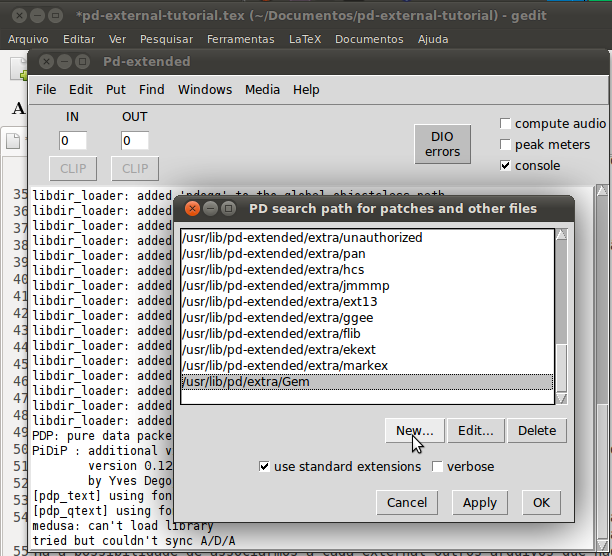
\includegraphics[scale=\Mysize]{path}
  \caption{Adicionando o diretório de um \external ao caminho de busca do Pure Data.}
  \label{fig:search-path}
\end{figure}

Para carregar uma biblioteca de \externals (mais de um \external no mesmo
arquivo-fonte), é possível indicar o nome da bibliotecai na linha
de comando do Pure Data utilizando a opção \texttt{-lib <biblioteca>}, ou
também graficamente através do menu \texttt{File} $\rightarrow$
\texttt{Startup...}, como pode ser visto na figura \ref{fig:lib}.

\begin{figure}[h!]
  \centering
  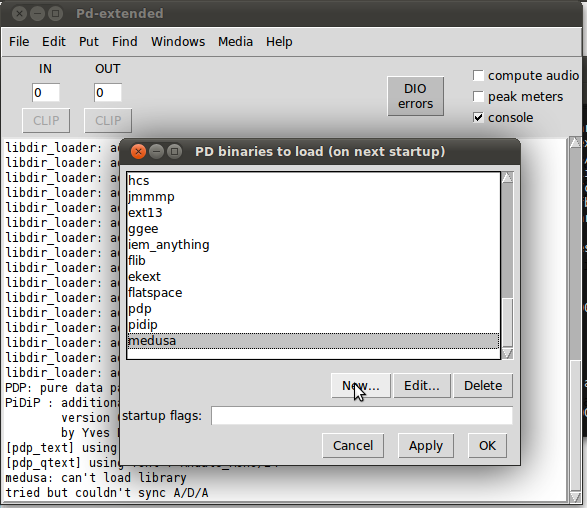
\includegraphics[scale=\Mysize]{startup}
  \caption{Adicionando uma biblioteca ao Pure Data.}
  \label{fig:lib}
\end{figure}

% -----+-----+-----+-----+-----+-----+-----+-----+-----+-----+-----+-----+-----+
%      |     |     |     |     |     |     |     |     |     |     |     |     |
% -----+-----+-----+-----+-----+-----+-----+-----+-----+-----+-----+-----+-----+
\section{Exemplos}
Este tutorial é acompanhado de diversos exemplos de \externals que ilustram o
conteúdo coberto pelo mesmo.
Vale lembrar que muitos destes objetos são de utilidade duvidosa e servem apenas
como exemplos didáticos.
Os arquivos de exemplo estão no mesmo repositório que este material.
No início de cada capítulo há uma caixa apresentando quais exemplos podem ser
utilizados.

% ----------------------------------------------------------------------------
% O básico de um \external
% ----------------------------------------------------------------------------

\chapter{O básico de um \external}

Escrever um \external significa seguir as recomendações da API. Peço ao leitor
bastante paciência pois este tutorial pretende andar um pouco devagar para
mostrar os passos da escrita de um \external.

\section{Um \external simples}

Como dissemos anteriormente, a arquitetura do Pure Data é organizada de acordo
com o paradigma de orientação a objetos: cada objeto gráfico do Pure Data
corresponde a uma instância de uma classe. Neste sentido, um \external está
associado a uma estrutura de dados que representa uma classe em C. Para cada
classe é necessário haver métodos de instanciação, destruição, processamento
de sinais, tratamento de mensagens, etc.

A infraestrutura mínima para o funcionamento de uma classe consiste em uma
estrutura de dados para a representação da classe, que deve ser chamada
\texttt{t\_<external>}, e dois métodos obrigatórios: \texttt{<external>\_setup()}
e \texttt{<external>\_new()}. A convenção de nomes utilizada no Pure Data é de
que toda função deve ser nomeada da forma
\texttt{<external>\_<metodo>(<argumentos>)}.

A estutura de dados que representa uma classe do Pure Data deve
obrigatoriamente possuir o primeiro atributo do tipo \texttt{t\_object}, no
qual é armazenado o objeto instanciado no momento da instanciação.  Outros
atributos podem ser adicionados a esta estrutura de maneira que cada instância
da mesma classe possua os atributos necessários para seu funcionamento. Uma
classe que acessa um arquivo, por exemplo, pode possuir como atributos uma
string para guardar o caminho e um inteiro para guardar o descritor do
arquivo.

Um exemplo de estrutura de dados para representação de uma classe chamada
\texttt{example01} consiste no seguinte:

\vspace{1em}
\begin{lstlisting}
static t_class *example01_class;

typedef struct _example01 {
  t_object x_obj;
} t_example01;
\end{lstlisting}

Sempre que um \external é carregado pelo Pure Data, o método de nome
\texttt{<external>\_setup()} é executado. No exemplo dado acima, o Pure
Data irá procurar, no arquivo binário \texttt{example01.pd\_linux} que contém
a biblioteca compartilhada, o método de nome \texttt{example01\_setup(void)}.
Este método é utilizado para realizar a inicialização da classe, informando ao
Pure Data da existência de uma nova classe no sistema e associando a ela os
métodos de instanciação e destruição, além de outras informações:

\vspace{1em}
\begin{lstlisting}
void example1_setup(void) {
  example1_class = class_new(
    gensym("example1"),         // Nome simbolico
    (t_newmethod) example1_new, // Construtor
    0,                          // Destrutor
    sizeof (t_example1),        // Tamanho dos atributos
    CLASS_NOINLET,              // Flags da classe
    0                           // Tipos dos argumentos
  );
}
\end{lstlisting}

Dentro do método \texttt{<external>\_setup()} não há limite para o número de
classes a definir, de forma que é possível definir apenas uma classe (como no
exemplo 01) ou uma biblioteca inteira com várias classes (como no exemplo 03).
A introdução de uma nova classe no sistema é realizada pela função
\texttt{class\_new()}. São parâmetros da função \texttt{class\_new()}:

\begin{itemize}
\item Nome simbólico da classe.
\item Método construtor de um objeto.
\item Método destrutor de um objeto.
\item Tamanho do espaço de dados dos atributos de um objeto.
\item Flags que definem a representação gráfica do objeto.
\item Tipos dos parâmetros a serem passados para o construtor quando da
      instanciação de um objeto (veja o próximo capítulo).
\end{itemize}

É necessário terminar a lista de tipos de parâmetros com um número inteiro 0,
para indicar ao Pure Data que a lista de tipos terminou. Consulte a
documentação da função \texttt{class\_new()} para mais
detalhes\footnote{http://pdstatic.iem.at/externals-HOWTO/node9.html\#SECTION00092100000000000000}.

O método \texttt{<external>\_new()}, que foi associado como método de
instanciação de objetos na chamada de \texttt{class\_new()}, realiza a
instanciação de objetos propriamente dita. Neste método, além da instanciação
de um novo objeto através da função \texttt{pd\_new()}, é possível definir os
valores dos atributos da estrutura de dados da classe e também inicializar
quaisquer outros contextos que sejam necessários, como por exemplo abrir
arquivos, preencher vetores, alocar memória, etc.

\vspace{1em}
\begin{lstlisting}
// Construtor da classe
void * example01_new(void) {
    t_example1 *x = (t_example1 *) pd_new(example1_class);
    return (void *) x;
}
\end{lstlisting}

Após a criação da estrutura de dados dos métodos da forma mencionada acima, a
compilação realizada da forma descrita na seção \ref{sec:compiling}, e a
criação do objeto no Pure Data como descrito na seção \ref{sec:using}, o
resultado pode ser visto na figura \ref{fig:example01working}.

\begin{figure}[h!]
  \centering
  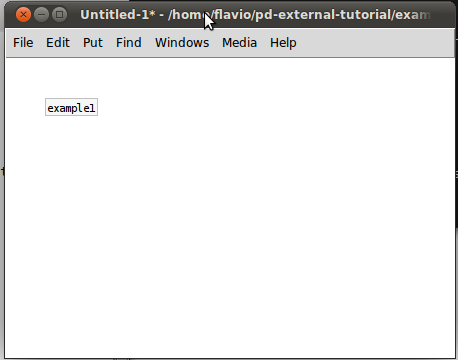
\includegraphics[width=0.7\textwidth]{example1}
  \caption{Nosso primeiro \external do PD. Ainda inútil. :-$\left.\right)$}
  \label{fig:example01working}
\end{figure}

\section{Uma biblioteca simples}

Um mesmo método \texttt{<external>\_setup()} pode definir várias classes
diferentes. A isto damos o nome de biblioteca. Para isto, o método
\texttt{<external>\_setup()} terá o mesmo nome do arquivo com a biblioteca mas
as classes  podem ter outros nomes. Veja o exemplo 03.

\vspace{1em}
\begin{lstlisting}
void example3_setup(void) {
    post("Initializing my library");

    myobj1_class = class_new(gensym("myobj1"),
            (t_newmethod) myobj1_new, // Constructor
            0,
            sizeof (t_myobj1),
	    CLASS_NOINLET,
            0);
    class_sethelpsymbol(myobj1_class, 
	gensym("myobj1-help"));

    myobj2_class = class_new(gensym("myobj2"),
            (t_newmethod) myobj2_new, // Constructor
            0,
            sizeof (t_myobj2),
	    CLASS_NOINLET,
            0);
    class_sethelpsymbol(myobj2_class, 
	gensym("myobj2-help"));

}
\end{lstlisting}

Se o arquivo foi feito corretamente, compilado corretamente e adicionado ao
caminho do PureData, teremos o resultado.

\begin{figure}[h!]
	\centering
	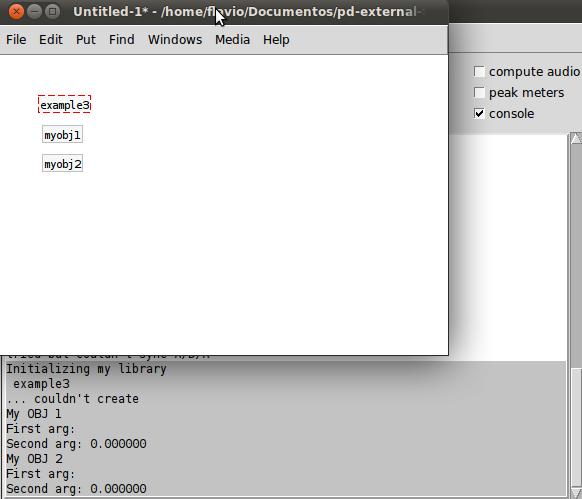
\includegraphics[width=0.7\textwidth]{example3}
	\caption{Nosso primeiro \external do PD. Ainda inútil.:-)}
\end{figure}


No caso da biblioteca, podemos ter um arquivo de help para cada \external. Esta
associação é feita pela função:

\vspace{1em}
\begin{lstlisting}
class_sethelpsymbol(myclass_class, gensym("my_class-help"));
\end{lstlisting}

Um objeto pode ainda ter outros nomes ou alias. Para definir isto podemo utilizar a função class\_addcreator. Veja o exemplo:

\vspace{1em}
\begin{lstlisting}
class_addcreator((t_newmethod)medusa_new, gensym("med"), 0);
\end{lstlisting}

\section{Variáveis globais}

Você pode usar uma variável global para armazenar dados pelos seus \externals.
Esta variável será visível para todas as intâncias do \external e todas podem
alterar seu valor. Isto pode ser útil ou um desastre. (Veja o exemplo16).

\vspace{1em}
\begin{lstlisting}
int count = 0;

void * example16_new(void) {
    t_example16 *x = (t_example16 *) pd_new(example16_class);
    post("Counter value: %d",count);
    count++;
    return (void *) x;
}
\end{lstlisting}

\begin{figure}[h!]
	\centering
	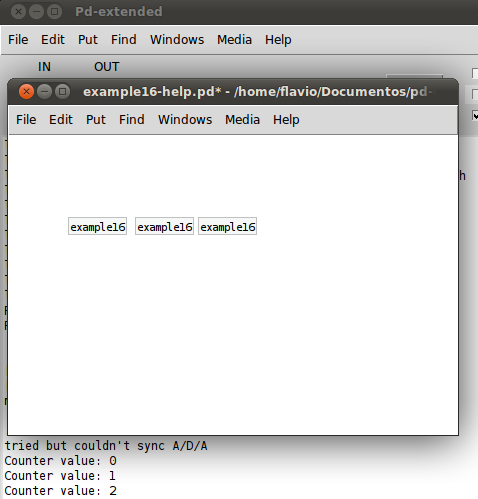
\includegraphics[width=0.7\textwidth]{example16}
	\caption{Repare no output da janela principal.}
\end{figure}

Caso isto não seja desejável, o ideal é colocar suas variáveis dentro da
struct do objeto. Assim cada instância terá seu próprio contador.

\vspace{1em}
\begin{lstlisting}
static t_class *example_class;

typedef struct _example {
    t_object x_obj;
    t_int counter;
} t_example;

void * example_new(void) {
    t_example *x = (t_example *) pd_new(example_class);
    post("Counter value: %d",x->counter);
    counter++;
    return (void *) x;
}

\end{lstlisting}


% ----------------------------------------------------------------------------
% OS TIPOS DE DADOS DO PD
% ----------------------------------------------------------------------------

\chapter{Os tipos de dados do PD}

Você pode usar os tipos de dados padrões do C, como int, float ou char. O
difícil é entender o que chamamos de tipos de dados padrões do C já que estes
tipos podem variar de acordo com o sistema operacional, compilador e outras
coisas. Por isto, para o external possa se comportar da mesma maneira em
qualquer sistema, é bastante recomendado que usemos os tipos do pure data.

Os tipos do pure data nada mais são que um


% ----------------------------------------------------------------------------
% CONSTRUTOR E DESTRUTOR
% ----------------------------------------------------------------------------

\chapter{Construtor e destrutor}

O Construtor de um objeto pode receber parâmetros. Estes parâmetros são
ilustrados abaixo.

\begin{figure}[h!]
	\centering
	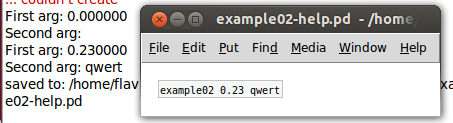
\includegraphics[width=0.7\textwidth]{example2}
	\caption{External recebendo parâmetros. Note a tela de saída no fundo da imagem.}
\end{figure}

\section{Construtor}

Parâmetros de inicialização no construtor podem permitir que inicializemos o
external com determinados valores. Isto é feito definindo os parâmetros no
métodos class\_new() quanto na definição da função construtora. (Veja o
exemplo02).

\begin{lstlisting}
// Constructos of the class
void * example2_new(t_symbol * arg1, t_floatarg arg2) {
    t_example2 *x = (t_example2 *) pd_new(example2_class);
    post("First arg: %s", arg1->s_name);
    post("Second arg: %f", arg2);
    return (void *) x;
}

void example2_setup(void) {
    example2_class = class_new(gensym("example2"),
            (t_newmethod) example2_new, // Constructor
            0,
            sizeof (t_example2),
	    CLASS_NOINLET,
            A_DEFFLOAT, // First Constructor parameter
            A_DEFSYMBOL, // Second Constructor parameter
            0);
}
\end{lstlisting}

Notem que os parâmetros são definidos com um tipo e são recebidos com outro.
Como explicado na seção \ref{sec:mensagens}, todos os dados que não
correspondem a sinais de áudio são transmitidos como mensagens, compostas de
átomos. Para ver os tipos de átomo que podem ser utilizados na passagem de
parâmetros, veja a seção \ref{sec:atomos}.

Para aceitar qualquer tipo de átomo na passagem de um parâmetro específico,
utilize o tipo de átomo \texttt{A\_GIMME} (veja o exemplo09).

\begin{lstlisting}
// Constructor of the class
void * example9_new(t_symbol *s, int argc, t_atom * argv) {
   t_example9 *x = (t_example9 *) pd_new(example9_class);
   post("%d parameters received",argc);
   return (void *) x;
}

void example9_setup(void) {
   example9_class = class_new(gensym("example9"),
     (t_newmethod) example9_new, // Constructor
     (t_method) example9_destroy, // Destructor
     sizeof (t_example9),
     CLASS_NOINLET,
     A_GIMME, // Allows various parameters
     0); // LAST argument is ALWAYS zero
}
\end{lstlisting}

Quando utilizamos o tipo de átomo \texttt{A\_GIMME} o método construtor
funciona como uma função \texttt{main()} em C: ela recebe os parâmetros
\texttt{argc}, que indica o número de átomos na lista, e \texttt{*argv}, que
aponta para a lista de átomos de fato. Veja o exemplo na figura
\ref{fig:construtor-parametros}.

\begin{figure}[h!]
\centering
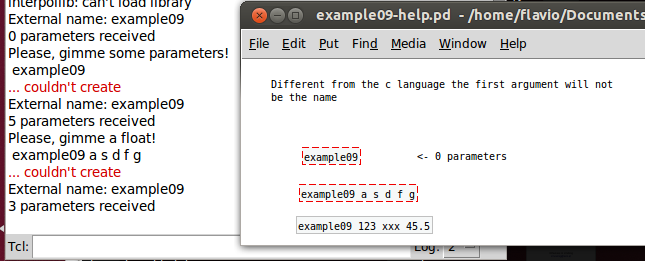
\includegraphics[width=0.7\textwidth]{example9}
\caption{Diferente da linguagem C, o primeiro parâmetro não é o nome do external.}
\label{fig:construtor-parametros}
\end{figure}

Note que o Pure Data não obriga que o usuário passe parâmetros para o objeto. É
como se todo construtor, independentemente de como ele está definido, aceitasse
sua instanciação vazia. Cabe ao programador verificar se os parâmetros
recebidos são em quantidade, tipo e valor esperado e, caso não seja, abortar a
construção do objeto e não retornar sua instância.

\section{Destrutor}

O destrutor de uma classe permite liberar alguma memória eventualmente alocada
pelo construtor ou por outras funções do \external (veja o exemplo 07).

\begin{lstlisting}
// Destroy the object
void example9_destroy(t_example9 *x) {
  post("You say good bye and I say hello");
}

void example9_setup(void) {
   example9_class = class_new(gensym("example9"),
     (t_newmethod) example9_new, // Constructor
     (t_method) example9_destroy, // Destructor
     sizeof (t_example9),
     CLASS_NOINLET,
     A_GIMME, // Allows various parameters
     0); // LAST argument is ALWAYS zero
}
\end{lstlisting}

A liberação da memória pode ser feita utilizando a função \texttt{freebytes()}
definida na API do Pure Data.

\begin{lstlisting}
void freebytes(void *x, size_t nbytes)
\end{lstlisting}


\section{Inlets e Outlets}


\begin{frame}{Inlets e outlets}
\begin{figure}[ht!]
\centering
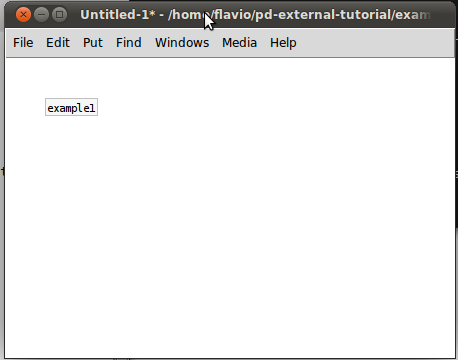
\includegraphics[height=0.6\textheight]{example1}
\caption{Para que serve isso!?}
\end{figure}
\end{frame}


\begin{frame}{Inlets passivos (1/3)}
\begin{figure}[h!]
\centering
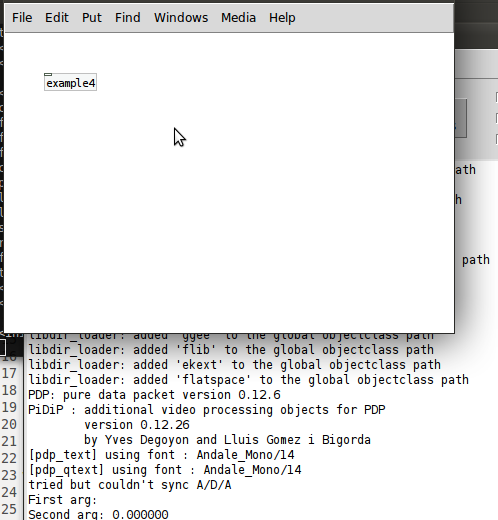
\includegraphics[height=0.8\textheight]{example4}
\label{fig:inlet-passivo}
\end{figure}
\end{frame}


\begin{frame}[fragile]{Inlets passivos (2/3)}
\begin{lstlisting}
static t_class *example4_class;

typedef struct _example4 {
  t_object x_obj;
  t_float my_float;
} t_example4;

// Constructor of the class
void *example4_new(t_symbol *arg1, t_floatarg arg2) {
  t_example4 *x = (t_example4*)pd_new(example4_class);
  post("First arg: %s", arg1->s_name);
  post("Second arg: %f", arg2);
  floatinlet_new(&x->x_obj, &x->my_float);
  return (void *) x;
}
\end{lstlisting}
\end{frame}


\begin{frame}{Inlets passivos (3/3)}
As funções para criar inlets passivos dos tipos mais comuns são:
\begin{itemize}
\item \texttt{floatinlet\_new(t\_object *owner, t\_float *fp)}
\item \texttt{symbolinlet\_new(t\_object *owner, t\_symbol **sp)}
\item \texttt{pointerinlet\_new(t\_object *owner, t\_gpointer *gp)}
\end{itemize}
\end{frame}


\begin{frame}{Inlets ativos (1/2)}
\begin{figure}[h!]
\centering
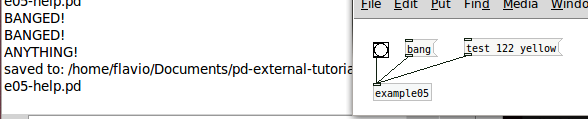
\includegraphics[width=0.7\textwidth]{example5}
\caption{Inlets ativos.}
\label{fig:inlet-ativo}
\end{figure}
\end{frame}


\begin{frame}[fragile]{Inlets ativos (2/2)}
\begin{lstlisting}[language=C]
// inlet-methods receive the object as first argument.
void example5_bang(t_example5 *x) { 
  post("BANGED!");
  post("My_float value: %f",x->my_float);
}

void example5_anything(t_example5 *x, t_symbol *s, int argc, t_atom *argv){
  post("ANYTHING!");
}

void example5_setup(void) {
  example5_class = class_new(gensym("example5"),
    (t_newmethod) example5_new, // Constructor
    0,  sizeof (t_example5), CLASS_DEFAULT,
    0); // LAST argument is ALWAYS zero
  class_addbang(example5_class, example5_bang);
  class_addanything(example5_class, example5_anything);
}
\end{lstlisting}
\end{frame}

\begin{frame}{Tratamento de mensagens (1/4)}
\begin{figure}[h!]
\centering
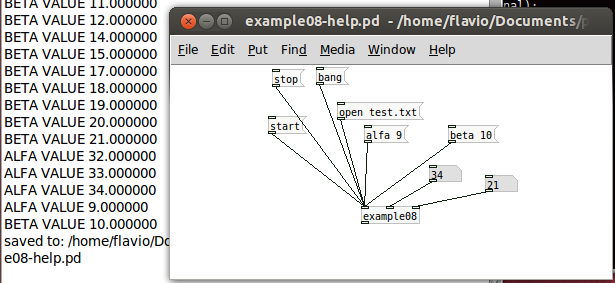
\includegraphics[width=0.7\textwidth]{example8}
\label{fig:inlet-ativo}
\end{figure}
\end{frame}

\begin{frame}[fragile]{Tratamento de mensagens (2/4)}
\lstinputlisting[name=Exemplo 08,linerange=47-61]{../examples/src/example08.c}
\end{frame}


\begin{frame}[fragile]{Tratamento de mensagens (3/4)}
\lstinputlisting[name=Exemplo 08,linerange=17-25,firstnumber=last]{../examples/src/example08.c}
\end{frame}


\begin{frame}[fragile]{Tratamento de mensagens (4/4)}
\lstinputlisting[name=Exemplo 08,linerange=27-45,firstnumber=last]{../examples/src/example08.c}
\end{frame}


\begin{frame}{Outlets (1/4)}
\begin{figure}[h!]
\centering
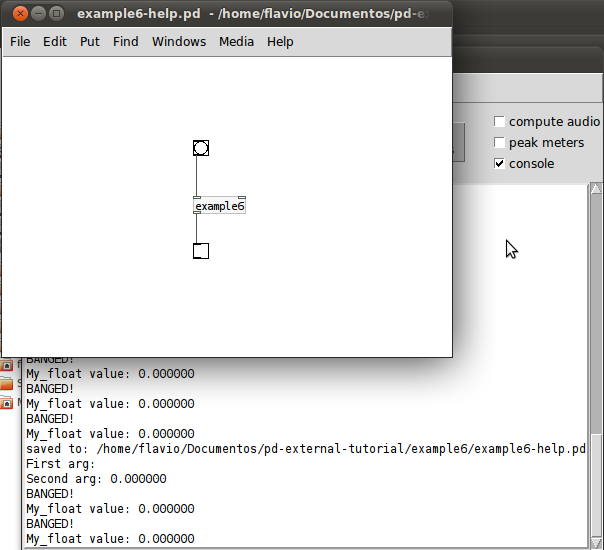
\includegraphics[width=0.7\textwidth]{example6}
\caption{Um external bem útil que recebe um bang e envia um bang.}
\label{fig:outlet-bang}
\end{figure}
\end{frame}


\begin{frame}{Outlets (2/4)}
\lstinputlisting[name=Exemplo 06,linerange=35-45]{../examples/src/example06.c}
\end{frame}


\begin{frame}{Outlets (3/4)}
\lstinputlisting[name=Exemplo 06,linerange=23-33,firstnumber=last]{../examples/src/example06.c}
\end{frame}


\begin{frame}{Outlets (4/4)}
\lstinputlisting[name=Exemplo 06,linerange=6-21,firstnumber=last]{../examples/src/example06.c}
\end{frame}


% ----------------------------------------------------------------------------
% DSP
% ----------------------------------------------------------------------------

\chapter{Processamento de Sinais Digitais}

\todo{Precisa mudar o nome dos exemplos para exemplo$\sim$. Neste caso, a função setup deve ser renomeada para "tilde\_setup")}

Enfim chegamos no processamento de áudio propriamente dito: \emph{Digital
Signal Processing} ou processamento de sinal digital. O Pure Data possui
inlets e outlets específicos para o processamento de sinal. É fácil
reconhecer: eles são pintados de cinza escuro.

\begin{figure}[h!]
\centering
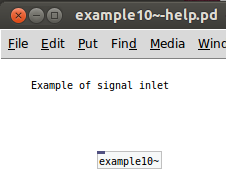
\includegraphics[width=0.7\textwidth]{example10}
\caption{Primeiro Inlet DSP}
\end{figure}

\section{Primeiro inlet para DSP}

Para realizar DSP no Pure Data é necessário alguns cuidados (veja o exemplo
10). Primeiramente, é necessário possuir na estrutura de dados um atributo do
tipo \texttt{t\_float} para armazenar o valor de entrada do inlet.

\lstinputlisting[name=Exemplo 10,linerange=6-9]{../examples/src/example10.c}

Se o \external necessita de apenas um inlet DSP, a macro
\texttt{CLASS\_MAINSIGNALIN()} define um inlet DSP no primeiro inlet da
esquerda. Para esta macro funcionar, é necessário que a classe seja do tipo
\texttt{CLASS\_DEFAULT}, e que um método seja associado à mensagem ``dsp", de
forma que será executado quando o DSP for iniciado. A forma de declaração de
outros inlets DSP será vista logo adiante.

\lstinputlisting[name=Exemplo 10,linerange=36-46,firstnumber=last]{../examples/src/example10.c}
 
O próximo passo é definir o método DSP que associamos na função
\texttt{\_setup()}:

\lstinputlisting[name=Exemplo 10,linerange=31-34,firstnumber=last]{../examples/src/example10.c}

Todo método de processamento de sinais associado através da função
\texttt{dsp\_add()} será executado em todo ciclo DSP enquanto o processamento
de sinais estiver ligado para o Pure Data ou para aquela janela específica,
através do objeto \texttt{switch~}. Por isto, cuidado com alocações de
memória, inicialização de variáveis, etc.

Neste exemplo, o método \texttt{example10\_perform()} é associado ao
processamento de áudio do Pure Data e será chamada em cada execução do ciclo
DSP com 3 argumentos: o endereço para o sinal de entrada
(\texttt{sp[0]->s\_vec}), a quantidade de amostras no bloco
(\texttt{sp[0]->s\_n}), e o endereço da estrutura que contém sua instância
(\texttt{x}).

Podemos passar para o método perform quaisquer parâmetros em qualquer ordem.
Só é importante e óbvio que devemos lembrar quais parâmetros foram passados e
em qual ordem. O próximo passo é criar o método perform propriamente dito.

\lstinputlisting[name=Exemplo 10,linerange=23-29,firstnumber=last]{../examples/src/example10.c}

\todo{Pergunta: O que raios há na posição w[0]? Resposta: o endereço da própria função
perform.}

O método perform receberá como parâmetro um vetor com os valores definidos no
método \texttt{dsp\_add()}. A posição 0 deste vetor sempre conterá o endereço
para a própria função \texttt{\_perform()}. Nas próximas posições devemos rever
o que definimos na função DSP acima. Na posição 1, o sinal de entrada;
na posição 2 o tamanho do vetor de entrada e na posição 3 a estrutura de dados
correspondente ao objeto. Note que podemos enviar estes dados em outra ordem ou
ainda enviar outros dados para a função \texttt{perform()}.
Este método deve retornar a próxima posição do vetor, ou seja, o endereço dado 
na chamada somado com a quantidade de atributos do método mais um.

\section{Vários inlets DSP}

É possível definir vários inlets de DSP para um \external (veja o exemplo 11).
A criação de inlets adicionais não é feita no método \texttt{\_setup()} mas
sim no construtor do objeto. Quanto ao primeiro inlet, só é necessário
definí-lo explicitamnete no construtor se a classe não for do tipo
\texttt{CLASS\_DEFAULT}.

\lstinputlisting[name=Exemplo 11,linerange=12-19]{../examples/src/example11.c}

Neste caso, a utilização do método \texttt{class\_addmethod} é exatamente
igual à anterior, a menos de uma mudança na quantidade de parâmetros por causa
da quantidade de inlets:

\lstinputlisting[name=Exemplo 11,linerange=36-38,firstnumber=last]{../examples/src/example11.c}

Note que precisamos agora alterar a quantidade de parâmetros passadas ao método
\texttt{\_perform()}, que ficará assim:

\lstinputlisting[name=Exemplo 11,linerange=26-34,firstnumber=last]{../examples/src/example11.c}

Neste ponto, este external deve ter uma aparência como na figura
\ref{fig:inlets-dsp}.

\begin{figure}[h!]
\centering
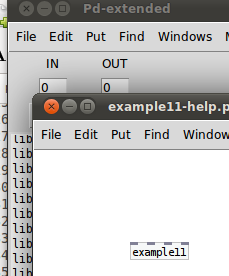
\includegraphics[width=0.3\textwidth]{example11}
\caption{Vários inlets DSP.}
\label{fig:inlets-dsp}
\end{figure}

\section{Primeiro outlet DSP}

A criação dos outlets é feita no construtor do external (veja o exemplo 12) e
não é necessário adicionar os outlets à estrutura da classe.

\lstinputlisting[name=Exemplo 12,linerange=12-20]{../examples/src/example12.c}

A definição do método \texttt{\_perform()} será idêntica ao do exemplo
anterior, quando criamos quatro inlets:

\lstinputlisting[name=Exemplo 12,linerange=37-39,firstnumber=last]{../examples/src/example12.c}

O método perform também será quase idêntico ao do exemplo anterior, porém
recebendo quatro outlets:

\lstinputlisting[name=Exemplo 12,linerange=27-35,firstnumber=last]{../examples/src/example12.c}

O resultado pode ser visto na figura \ref{fig:primeiro-outlet}.

\begin{figure}[h!]
\centering
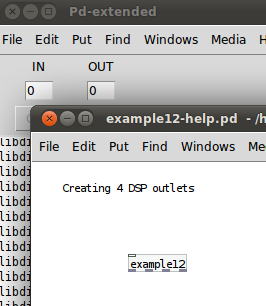
\includegraphics[width=0.3\textwidth]{example12}
\caption{Primeiro Outlet DSP.}
\label{fig:primeiro-outlet}
\end{figure}

\section{Inlets e outlets DSP}

Nosso próximo exemplo (veja o exemplo 13) mistura no mesmo objeto inlets e
outlets DSP, o que é bastante comum. Neste ponto, deve estar mais ou menos
claro como é feita a construção de um objeto assim. Não é necessário guardar 
os endereços dos inlets e outlets na estrutura de dados que representa o objeto. 
É necessário apenas criar os inlets e outlets no construtor (lembre-se que o 
primeiro inlet já foi criado no método setup. Ele é mágico!).

\lstinputlisting[name=Exemplo 13,linerange=12-25]{../examples/src/example13.c}

No método seguinte associamos o método \texttt{\_perform()} à cadeia DSP do
Pure Data:

\lstinputlisting[name=Exemplo 13,linerange=46-48,firstnumber=last]{../examples/src/example13.c}

No método \texttt{\_perform()} recebemos como argumento um bloco de memória
que contém primeiro os buffers de entrada e em seguida os buffers de saída:

\lstinputlisting[name=Exemplo 13,linerange=32-44,firstnumber=last]{../examples/src/example13.c}

O resultado pode ser visto na figura \ref{fig:varios-inlets-outlets}.

\begin{figure}[h!]
\centering
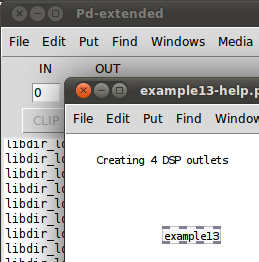
\includegraphics[width=0.3\textwidth]{example13}
\caption{Vários inlets e outlets DSP.}
\label{fig:varios-inlets-outlets}
\end{figure}

\section{Inlets e outlets DSP criados dinamicamente}

É possível definir através de parâmetros para o construtor a quantidade de
inlets e/ou outlets DSP que um external deve possuir. Isso significa que o
número de inlets e outlets é definido dinamicamente, em tempo de execução,
através de um argumento. Para isto, existe mais de uma possibilidade de
implementação.

A primeira possibilidade consiste em passarmos para o construtor a informação
de quantos inlets e outlets teremos na função dsp (veja o exemplo
17) e armazenarmos na estrutura de dados que contém o objeto do \external.

\lstinputlisting[name=Exemplo 17,linerange=6-25]{../examples/src/example17.c}

Na passagem de parâmetro para o DSP usamos estas variáveis para contar quantos
parâmetros serão usados.

\lstinputlisting[name=Exemplo 17,linerange=33-48,firstnumber=last]{../examples/src/example17.c}

A segunda opção é usar outro método que baseia-se no modelo de alocação de
memória do pd. Criamos um vetor e apontamos este vetor para o dado da entrada
/ saída do external. Assim podemos utilizar a estrutura amarrada ao external
para produzir / consumir o dado. Veja o exemplo 19.

\lstinputlisting[name=Exemplo 19,linerange=44-53]{../examples/src/example19.c}

Neste ponto, esta solução é bastante parecida com a anterior e poderia ser usada também com uma quantidade
variável de outlets. A alteração está na estrutura da classe.

\lstinputlisting[name=Exemplo 19,linerange=6-10,firstnumber=last]{../examples/src/example19.c}

Ok, 64 não é um número mágico de verdade. Ele é o tamanho de bloco padrão do
Pure Data. Para que esta solução seja genérica o suficiente é melhor usar a
função \texttt{sys\_getblksize()} para obter o tamanho do bloco e alocar
a quantidade correta de espaço. Da forma em que está, corremos o risco de
obter erros de leitura ou escrita em lugares sem permissão. 

\lstinputlisting[name=Exemplo 19,linerange=14-22,firstnumber=last]{../examples/src/example19.c}

Como no exemplo anterior, o construtor cria a quantidade de outlets passada
como argumento na criação do objeto. Aqui, poderíamos utilizar
\texttt{malloc()} para alocar o vetor com os dados de maneira inteligente ao
invés de usar o 64 mágico.

\lstinputlisting[name=Exemplo 19,linerange=36-41,firstnumber=last]{../examples/src/example19.c}

O método DSP não fará mais que passar o próprio objeto ao método
\texttt{\_perform()}. Na verdade, poderia não passar nem o objeto.

\lstinputlisting[name=Exemplo 19,linerange=30-34,firstnumber=last]{../examples/src/example19.c}

A função perform não precisa fazer nada mais que despertar o processo
consumidor e liberar o processamento no Pure Data. E este é um ponto que
considero importante para levantar outro questionamento.

O Pd precisa que o processamento dos blocos termine em determinado tempo. Qual
seria este tempo? Para um bloco de 64 amostras e taxa de amostragem 44.100
amostras por segundo, é necessário que todo o processamento para um bloco
termine em um pouco mais de 1 milisegundo. Parece rápido mas seu computador é
mais rápido que isto. Criar um processo consumidor que libere o bloco de 
processamento pode ser uma abordagem melhor para processos baseados em fluxo,
como escrita em arquivos. Para isto precisamos utilizar outra função em outra 
thread e este é nosso próximo assunto.

\todo{Vale a pena mostrar como fazer o loop entre as amostras ou é óbvio?}

% ----------------------------------------------------------------------------
% MULTITHREADING
% ----------------------------------------------------------------------------

\chapter{Multithreading}

Como vimos no capítulo anterior, o bloco de processamento do Pd possui um
limite de tempo para a execução. É possível utilizar threads para separar
processos que consumam mais tempo do que o o período do bloco DSP, como por
exemplo no vaso de processos do tipo produtor/consumidor.

A programação multithread não é exatamente comum no Pure Data mas pode ser
útil para várias coisas como escrita em arquivo, envio de dados para a rede ou
atualização da interface gráfica (como veremos no próximo capítulo).

Apesar de existirem várias bibliotecas para programação paralela, como por
exemplo a simples utilização do comando fork do GNU/Linux, é desejável que os
externals do Pure Data sejam compatíveis com diversos sistemas operacionais.
Nos repositórios do Miller Puckette, autor do Pure Data, encontramos patches
nos quais ele utiliza threads POSIX implementadas pela biblioteca
\texttt{pthread} \footnote{Para maiores informações, visite:
https://computing.llnl.gov/tutorials/pthreads/}.

Note que esta solução, que em muito se aproxima da última forma de criar
inlets e outlets DSP implica em não trabalharmos mais em tempo real.
Implementações deste tipo não podem ser pensadas para processamentos aonde a
entrada de áudio será processada e devolvida na saída de áudio no mesmo bloco
de processamento do Pd.

\section{Criando threads}

Para utilizar a biblioteca de threads do POSIX é necessário incluir o arquivo
de cabeçalho correspondente. Em seguida, para armazenar as threads que
criamos, utilizamos uma variáveis que armazenam threads (veja o exemplo 20).

\begin{lstlisting}
#include <pthread.h>
...
typedef struct _example20 {
    t_object x_obj;
    pthread_t example20_thread;
} t_example20;

\end{lstlisting}

O próximo passo é criar uma função associada a esta thread e a enfim lançar a
thread. O lançamento da thread pode ser feito na função DSP. Isto implica
criar e iniciar uma thread nova em cada ciclo DSP do Pd.

\begin{lstlisting}
void * example20_thread_function(void * arg) {
  t_example20 *x = (t_example20 *) arg;
  while(1){
    // DO SOMETHING
    printf("Threading running!\n");
    sleep(1);
  }
  return 0;
}

static void example20_dsp(t_example20 *x, t_signal **sp){
  pthread_create(&x->example20_thread, NULL, example20_thread_function, x);
  dsp_add(example20_perform, 1 , x);
}
\end{lstlisting}

A função de criação da thread recebe o endereço da variável aonde a thread
será armazenada, os atributos da thread sendo criada\footnote{No caso,
passando \texttt{NULL} serão utilizados os atributos padrão. Para uma lista
completa dos atributos, visite:
http://sourceware.org/pthreads-win32/manual/pthread\_attr\_init.html}, a
função de inicialização associada a esta thread e os argumentos passados para
esta função. 

Caso seja passado mais de um argumento, é recomendado que se crie uma
estrutura de dados e que esta seja passada como argumento para a thread.

\section{Gerenciamento de threads}

Há diversas funções para o gerenciamento de threads, definidas no arquivo de
cabeçalho \texttt{pthread.h}. Entre elas:

\begin{itemize}
\item \texttt{pthread\_detach(threadid)}: Indica para a implementação que o
armazenamento da thread pode ser recuperado quando a mesma se encontra
terminada
\item \texttt{pthread\_join(threadid,status)}: Indica para o trecho de código
que chamou a thread que o mesmo deve esperar que a mesma tenha terminado sua
execução.
\item \texttt{pthread\_exit(void *value\_ptr)}: Encerra a execução de uma
thread e libera sua alocação de memória.
\end{itemize}

Em princípio, threads POSIX não possuem funções para interromper e continuar a
execução. Apesar disto, é possível implementar estes comandos por meio de
mutexes, como veremos a seguir.

\section{Controle de concorrência}

Uma das dificuldades de utilização de threads é o controle da concorrência por
recursos entre threads. Em situações de race condition, é necessário que
controlemos o acesso de threads concorrentes a trechos de código que acessam
dados comuns. Isto é feito por meio de mutex (mutual exclusion), sistemas de
controle atômicos que garantem que apenas uma thread será executada sobre um
trecho de código por vez.

Um mutex é definido da seguinte forma:

\begin{lstlisting}
pthread_mutex_t lock = PTHREAD_MUTEX_INITIALIZER;
pthread_cond_t cond = PTHREAD_COND_INITIALIZER;
int play = 0;
\end{lstlisting}

O controle ao trecho de código pode ser feito da seguinte forma:

\begin{lstlisting}
for(;;) { /* Playback loop */
  pthread_mutex_lock(&lock);
  while(!play) { /* We're paused */
    pthread_cond_wait(&cond, &lock); /* Wait for play signal */
  }
  pthread_mutex_unlock(&lock);
  /* Continue playback */
}
\end{lstlisting}

\todo{Creio que seria mais útil um exemplo funcional...}

\section{Controle via Pure Data}
Além de podermos trabalhar threads para nosso external, na biblioteca do
Pd há funções para que possamos criar mutex no Pd. São elas:

\begin{itemize}
\item \texttt{void sys\_lock(void);}
\item \texttt{void sys\_unlock(void);}
\item \texttt{int sys\_trylock(void);}
\end{itemize}

% ----------------------------------------------------------------------------
% GUI
% ----------------------------------------------------------------------------

\chapter{Externals com GUI - Usando o Tcl/Tk}

O Pd permite que externals possuam interfaces gráficas mais rebuscadas que as simples
caixinhas que o mesmo desenha. Isto pode ser feito adicionando código Tcl/tk ao external.
Isto porque a GUI do próprio Pd é feita nesta linguagem.

\section{Iniciando no Tcl/Tk}

O Tcl (Tool Command Language) é uma linguagem de programação dinâmica bastante poderosa e simples de ser utilizada. 
Tk é um conjunto de ferramentas para construção de GUI de aplicações desktop e é a GUI padrão não apenas do TCL mas 
de várias outras linguagens e pode ser executada nativamente em vários sistemas operacionais modernos como Windows,
 Mac OS X, Linux, entre outros \footnote{Visite: http://www.tcl.tk/ para maiores informações}.

O Tk possui vários objetos prontos para GUI como botões, labels, janelas, checkbox, entre outros. Os objetos criados
devem ser armazenados em uma variável. Toda variável em Tk possui um nome que inicia com ponto (.). Após criar o objeto
e definir seus atributos, basta que o mesmo seja empacotado (pack).

\begin{lstlisting}
label .hello -text "Hello World"
pack .hello
\end{lstlisting}

Uma vez que um programa tk esteja pronto, basta salvá-lo com a extensão .tcl e utilizar um interpretador para executá-lo.
Um exemplo deste interpretador no Linux é o wish. Assim, salvando o exemplo anterior com o nome de helloWorld.tcl e executando

\begin{lstlisting}
wish helloWorld.tcl
\end{lstlisting}

Teremos o resultado:
\begin{figure}[ht!]
	\centering
	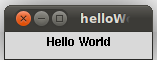
\includegraphics[width=0.7\textwidth]{helloWorld}
	\caption{Hello World no Tcl/Tk}
\end{figure}

No diretório tk deste tutorial temos exemplos mais interessantes de GUI com Tk mas a prática desta linguagem
vai além do escopo deste tutorial. Um tutorial mais completo de Tcl/Tk pode ser encontrado em 
\footnote{http://www.bin-co.com/tcl/tutorial/} e uma lista dos objetos e parâmetros pode ser encontrada em
\footnote{http://www.tkdocs.com/widgets/index.html}.

\section{Escrevendo externals com GUI}

A primeira necessidade para implementar um external com GUI é a inclusão da biblioteca g\_canvas.h. Esta biblioteca
encontra-se disponível em \footnote{http://www.koders.com/c/fid97160440CD236854358462C336536646E0933C46.aspx} e nela estarão
as funcionalidades necessárias para que o Pd desenhe nossas GUI. Veja que não queremos alterar a GUI do Pd mas
apenas fazer uma GUI para o external. Isto significa que teremos o cuidade de pedir ao Pd que desenhe nossa GUI.

O segundo passo é definirmos uma variável para armazenar o comportamento do nosso objeto (Veja o exemplo 14).

\begin{lstlisting}
t_widgetbehavior widgetbehavior; // This represents the external GUI
\end{lstlisting}

Nesta variável teremos as funções definidas para o que acontece com nosso objeto gráfico. Isto deve ser 
feito no método setup do objeto.

\begin{lstlisting}
void example14_setup(void) {
    example14_class = class_new(gensym("example14"),
            (t_newmethod) example14_new, // Constructor
            (t_method) example14_destroy, // Destructor
            sizeof (t_example14),
	    CLASS_DEFAULT,
	    A_GIMME, // Allows various parameters
            0); // LAST argument is ALWAYS zero

    // The external GUI rectangle definition
    widgetbehavior.w_getrectfn = my_getrect;
    //How to make ir visible / invisible
    widgetbehavior.w_visfn= my_vis;
    //what to do whe moved
    widgetbehavior.w_displacefn= my_displace;
    // What to do when selected
    widgetbehavior.w_selectfn= my_select;
    // What to do when active
    widgetbehavior.w_activatefn = my_activate;
    // What to do when deleted
    widgetbehavior.w_deletefn = my_delete;
    // What to do when clicked
    widgetbehavior.w_clickfn = my_click;

    // What about object properties?
    class_setpropertiesfn(example14_class, my_properties);
    // How to save its properties with the patch?
    class_setsavefn(example14_class, my_save);

    //Associate the widgetbehavior with the class
    class_setwidget(example14_class, &widgetbehavior);

}
\end{lstlisting}

Além de definir as funções callback da GUI é necessário associar o widgetbehavior a classe. Uma vez que isto
for feito, o Pd não mais irá renderizar a famosa caixinha. A partir disto a responsabilidade de renderizar a 
GUI passa a ser do programador.

Vamos ver as funções criadas para desenhar uma GUI.

\begin{lstlisting}
// THE BOUNDING RECTANGLE
static void my_getrect(t_gobj *z, t_glist *glist, int *xp1, int *yp1, int *xp2, int *yp2){
	// This function is always called. 
	// Better do not put a post here...
	// post("GETRECT");
	t_example14 *x = (t_example14 *)z;
 	*xp1 = x->x_obj.te_xpix;
 	*yp1 = x->x_obj.te_ypix;
 	*xp2 = x->x_obj.te_xpix + 30;
 	*yp2 = x->x_obj.te_ypix + 50;
}
\end{lstlisting}

Esta função recebe ponteiros para inteiros que deverão ser apontados para os valores que queremos definir como
o retângulo do nosso objeto. Veja que isto não é necessariamente o tamanho do retângulo do objeto gráfico mas aonde o mesmo
poderá ser clicado na tela. Um exemplo disto é o comentário do Pd. Apesar do mesmo as vezes ficar maior, sua área 
clicável é sempre um quadradinho na esquerda. Isto significa que nem sempre a representação gráfica da área do objeto
é a mesma da sua área de desenho.

\begin{lstlisting}
// MAKE VISIBLE OR INVISIBLE
static void my_vis(t_gobj *z, t_glist *glist, int vis){
	t_example14 *x = (t_example14 *)z;

	// takes the Canvas to draw a GUI
	t_canvas * canvas = glist_getcanvas(glist);

	if(vis){ // VISIBLE
	post("VISIBLE");

        sys_vgui(".x%lx.c create rectangle %d %d %d %d -tags %xrr -fill #FF0000\n",
		glist_getcanvas(glist),
		x->x_obj.te_xpix,
		x->x_obj.te_ypix,
		x->x_obj.te_xpix + 70,
		x->x_obj.te_ypix + 50,
		x
		);
       sys_vgui(".x%x.c create text %d %d -text {example14} -anchor w  -tags %xlb\n",
                canvas,
		x->x_obj.te_xpix + 2,
		x->x_obj.te_ypix + 12,
		x);
	}else{ // INVISIBLE
		post("INVISIBLE");
		sys_vgui(".x%x.c delete %xrr\n",canvas, x);
		sys_vgui(".x%x.c delete %xlb\n",canvas, x);
	}
//	canvas_fixlinesfor(glist, (t_text *)x);
}\end{lstlisting}

Deixar o objeto visível ou invisível significa pedir a GUI do Pd que desenhe ou apague um desenho.
Neste caso nosso desenho é um retângulo vermelho. Usamos o nome da própria instância como nome do
objeto Tk para evitar que sobrescrevamos o nome de algum outro componente gráfico do Pd. Também desenhamos
um texto com o nome do objeto pois o Pd não fará isto. Caso nosso objeto se torne invisível, temos de
remover ambos do canvas.

\begin{lstlisting}
// WHAT TO DO IF SELECTED?
static void my_select(t_gobj *z, t_glist *glist, int state){
 	t_example14 *x = (t_example14 *)z;
 	if (state) {
	post("SELECTED");
        sys_vgui(".x%x.c create rectangle %d %d %d %d -tags %xSEL -outline blue\n",
		glist_getcanvas(glist),
		x->x_obj.te_xpix,
		x->x_obj.te_ypix,
		x->x_obj.te_xpix + 70,
		x->x_obj.te_ypix + 50,
		x
		);
	}else {
	post("DESELECTED");
 	sys_vgui(".x%x.c delete %xSEL\n",glist_getcanvas(glist), x);
	}
}
\end{lstlisting}

O que acontece quando um objeto do Pd é selecionado? Ele ganha um contorno azul. O que acontece
quando nosso objeto é selecionado? Nada. Por isto desenhamos aqui um contorno azul. Quando ele
é deselecionado, removemos o contorno azul.

\begin{lstlisting}
// DISPLACE IT
void my_displace(t_gobj *z, t_glist *glist,int dx, int dy){
	post("MOVED");
	t_canvas * canvas = glist_getcanvas(glist);
	t_example14 *x = (t_example14 *)z;
	x->x_obj.te_xpix += dx; // x movement
	x->x_obj.te_ypix += dy; // y movement

        sys_vgui(".x%lx.c coords %xSEL %d %d %d %d \n", //MOVE O SELECIONADO
		canvas,
		x,
		x->x_obj.te_xpix,
		x->x_obj.te_ypix,
		x->x_obj.te_xpix + 70,
		x->x_obj.te_ypix + 50
		);
        sys_vgui(".x%x.c coords %xrr %d %d %d %d\n",canvas,x,x->x_obj.te_xpix,x->x_obj.te_ypix,x->x_obj.te_xpix + 70,x->x_obj.te_ypix + 50);
        sys_vgui(".x%x.c coords %xlb %d %d \n",canvas,x,x->x_obj.te_xpix + 2, x->x_obj.te_ypix + 12);

	canvas_fixlinesfor(glist, (t_text *)x);
}
\end{lstlisting}

O que fazer quando movemos um objeto. Aqui será necessário mover todos os objetos pois não temos um
container que possui todos os objetos. Inclusive é necessário mover o contorno azul que desenhamos
quando o mesmo se tornou selecionado.

\begin{lstlisting}
// What to do if activated?
static void my_activate(t_gobj *x, struct _glist *glist, int state){
	post("Activated");
}
\end{lstlisting}

O método será executado quando um objeto se tornar ativo.

\begin{lstlisting}
static int my_click(t_gobj *z, struct _glist *glist, int xpix, int ypix, int shift, int alt, int dbl, int doit){
	post("Clicked xpix:%d ypix:%d shift:%d alt:%d dbl:%d doit:%d", xpix,ypix, shift, alt, dbl, doit);
	return 0;
}
\end{lstlisting}

O método click é retornado com qualquer evento do mouse. Caso ele seja clicado, o mesmo receberá o valor 1 no parâmetro doit.
Vale lembrar que este método só será executado quando o Pd não estiver no modo de edição.

\begin{lstlisting}
static void my_delete(t_gobj *z, t_glist *glist){
	t_text *x = (t_text *)z;
	canvas_deletelinesfor(glist_getcanvas(glist), x);
	post("Object deleted!");
} 
\end{lstlisting}

Este método será o destrutor da GUI.

\begin{lstlisting}
void my_save(t_gobj *c, t_binbuf *b){
	post("SAVE");
}
\end{lstlisting}

Quando salvamos o \patch pode ser necessário armazenar parâmetros para recuperar nosso external
como GUI na mesma situação. Este método recebe um buffer aonde poderá armazenar dados que serão
devolvidos quando o mesmo for recriado. Note que isto não está associado com a GUI mas com a classe.

\todo{Nunca implementei Salvar. Parece legal...}


\begin{lstlisting}
void my_properties(t_gobj *c, t_glist *list){
	post("PROPERTIES");
}
\end{lstlisting}

Caso o usuário pressione o botão contrário ele pode alterar as propriedades do objeto. Este método
permite definir a lista de propriedades que o objeto aceita. Note que isto não está associado com a GUI
mas com a classe.

\todo{Ainda não implementei propriedades.}

Caso nosso objeto tenha sido criado corretamente, ele ficará como a seguir
\begin{figure}[h!]
	\centering
	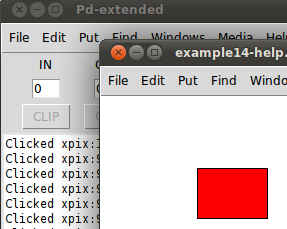
\includegraphics[width=0.7\textwidth]{example14}
	\caption{Adicionando GUI tk.}
\end{figure}

Note que este objeto foi definido em sua criação como um CLASS\_DEFAULT, o que implica que o mesmo possui
um inlet. Este inlet existe e está funcionando e aceitando conexões de outros objetos, mensagens e números.
Só não aceita conexões DSP pois as mesmas não foram definidas para este objeto. 
Mesmo assim o Pure Data não irá desenhá-lo pois precisamos definir tudo na GUI. Caso queira um
retângulo em cima para mostrar ao usuário que temos um inlet, temos que desenhá-lo, movê-lo quando necessário e 
também apagá-lo quando o objeto se tornar invisível.

\section{Adicionando componentes gráficos}

O Objeto Tk que o Pd nos disponibiliza é um canvas. Um canvas é, em princípio, uma tela de pintura. Em um canvas 
podemos adicionar linhas, ovals, pontos, textos, retângulos e janelas. É por se tratar de um canvas e não de uma
janela que não temos o conceito de um container para os objetos. Desta maneira, para adicionarmos um componente 
como um botão ou um slider, é necessário adicionarmos uma janela ao canvas para que a mesma abrigue este componente gráfico.
Há vários componentes gráficos que podem ser adicionados em um external. Vejamos um exemplo (exemplo 15).

\begin{lstlisting}
// MAKE VISIBLE OR INVISIBLE
static void my_vis(t_gobj *z, t_glist *glist, int vis){
	t_example15 *x = (t_example15 *)z;
	t_canvas * canvas = glist_getcanvas(glist);

	if(vis){ // VISIBLE
	// Define the tk/tcl commands / functions
	sys_vgui("proc do_something {} {\n set name [.x%x.c.s%xtx get]\n puts \"OIA: $name\" \n}\n",canvas,x);
	sys_vgui("proc do_otherthing {val} {\n set name [.x%x.c.s%xtx get]\n puts \"OIA: $name\" \n}\n",canvas,x);
    	// The text field
	sys_vgui("entry .x%x.c.s%xtx -width 12 -bg yellow \n", canvas,x);
	// The button
	sys_vgui("button .x%x.c.s%xbb -text {click} -command do_something\n", canvas,x);
	// The radio button	
	sys_vgui("radiobutton .x%x.c.s%xrb -value 1 -command do_something\n", canvas,x);
	// The h slider
	sys_vgui("scale .x%x.c.s%xsb -orient horizontal -command do_otherthing \n", canvas,x);
	// A checkbutton
	sys_vgui("checkbutton .x%x.c.s%xcb -foreground blue -background yellow -command do_something\n", canvas,x);
	// The red rectangle
        sys_vgui(".x%lx.c create rectangle %d %d %d %d -tags %xrr -fill #FF0000\n",
		glist_getcanvas(glist),
		x->x_obj.te_xpix,
		x->x_obj.te_ypix,
		x->x_obj.te_xpix + 170,
		x->x_obj.te_ypix + 150,
		x
		);
	// A window to the button (bb)
	sys_vgui(".x%x.c create window %d %d -anchor nw -window .x%x.c.s%xbb -tags %xbb\n",
		canvas,
		x->x_obj.te_xpix + 70,
		x->x_obj.te_ypix + 120,
		canvas,
		x,
		x);
	// A window to the radiobutton
	sys_vgui(".x%x.c create window %d %d -anchor nw -window .x%x.c.s%xrb -tags %xrb\n",
		canvas,
		x->x_obj.te_xpix + 70,
		x->x_obj.te_ypix,
		canvas,
		x,
		x);
	// A window to the combo box 
	sys_vgui(".x%x.c create window %d %d -anchor nw -window .x%x.c.s%xcb -tags %xcb\n",
		canvas,
		x->x_obj.te_xpix  + 100,
		x->x_obj.te_ypix,
		canvas,
		x,
		x);
	// A window to the slider button
	sys_vgui(".x%x.c create window %d %d -anchor nw -window .x%x.c.s%xsb -tags %xsb\n",
		canvas,
		x->x_obj.te_xpix,
		x->x_obj.te_ypix + 80,
		canvas,
		x,
		x);
	// A window to the text
	sys_vgui(".x%x.c create window %d %d -anchor nw -window .x%x.c.s%xtx -tags %xtx\n",
		canvas,
		x->x_obj.te_xpix,
		x->x_obj.te_ypix + 60,
		canvas,
		x,
		x);
	// a label field
       sys_vgui(".x%x.c create text %d %d -text {example15~} -anchor w  -tags %xlb\n",
                canvas,
		x->x_obj.te_xpix,
		x->x_obj.te_ypix + 40,
		x);

	}else{ // INVISIBLE
		sys_vgui(".x%x.c delete %xbb\n",canvas, x);
		sys_vgui(".x%x.c delete %xcb\n",canvas, x);
		sys_vgui(".x%x.c delete %xrb\n",canvas, x);
		sys_vgui(".x%x.c delete %xsb\n",canvas, x);
		sys_vgui(".x%x.c delete %xrr\n",canvas, x);
		sys_vgui(".x%x.c delete %xlb\n",canvas, x);
		sys_vgui(".x%x.c delete %xtx\n",canvas, x);
	}
}
\end{lstlisting}

Criamos os componentes gráficos e pedimos ao canvas para criar uma janela para que a mesma abrigue o componente.
Assim, na hora de remover podemos remover apenas a janela. O mesmo ocorre na hora de mover.
Note que além de adicionarmos componentes gráficos associamos eles a um comando. Este será nosso próximo tópico.

\begin{lstlisting}
void my_displace(t_gobj *z, t_glist *glist,int dx, int dy){
	t_canvas * canvas = glist_getcanvas(glist);
	t_example15 *x = (t_example15 *)z;
	x->x_obj.te_xpix += dx;
	x->x_obj.te_ypix += dy;

        sys_vgui(".x%lx.c coords %xSEL %d %d %d %d \n", //MOVE O SELECIONADO
		glist_getcanvas(glist),
		x,
		x->x_obj.te_xpix,
		x->x_obj.te_ypix,
		x->x_obj.te_xpix + 170,
		x->x_obj.te_ypix + 150
		);
        sys_vgui(".x%x.c coords %xrr %d %d %d %d\n",canvas,x,x->x_obj.te_xpix,x->x_obj.te_ypix,x->x_obj.te_xpix + 170,x->x_obj.te_ypix + 150);
        sys_vgui(".x%x.c coords %xbb %d %d \n",canvas,x,x->x_obj.te_xpix,x->x_obj.te_ypix);
        sys_vgui(".x%x.c coords %xcb %d %d \n",canvas,x,x->x_obj.te_xpix + 30,x->x_obj.te_ypix);
        sys_vgui(".x%x.c coords %xsb %d %d \n",canvas,x,x->x_obj.te_xpix,x->x_obj.te_ypix + 80);
        sys_vgui(".x%x.c coords %xtx %d %d \n",canvas,x,x->x_obj.te_xpix,x->x_obj.te_ypix + 120);
        sys_vgui(".x%x.c coords %xrb %d %d \n",canvas,x,x->x_obj.te_xpix + 60,x->x_obj.te_ypix);
        sys_vgui(".x%x.c coords %xlb %d %d \n",canvas,x,x->x_obj.te_xpix,x->x_obj.te_ypix + 40);

	canvas_fixlinesfor(glist, (t_text *)x);
}
\end{lstlisting}

\section{Adicionando comandos}

Os comandos dos nossos componentes gráficos podem ser recebidos e interagirem com o external assim como o
external consegue alterar os valores da GUI dependendo do que recebe em seus inlets. Veja o exemplo 21.

Para este exemplo, definimos na criação da classe no método setup() os métodos de retorno de nossa GUI.

\begin{lstlisting}
// depois associaremos estes "tipos" de mensagem aos inlets 2 e 3
    class_addmethod(example21_class, (t_method)example21_alfa,  gensym("alfa"), A_DEFFLOAT,0); 
    class_addmethod(example21_class, (t_method)example21_beta,  gensym("beta"), A_DEFFLOAT,0); 
// metodo do botao ok
    class_addmethod(example21_class, (t_method)example21_btok,gensym("btok"), A_DEFSYMBOL,0); 
\end{lstlisting}

No método vis da GUI, criamos comandos.

\begin{lstlisting}
	    sys_vgui("proc slide_alfa {val} {\n pd [concat example21%x alfa $val \\;]\n}\n",x);
	    sys_vgui("proc slide_beta {val} {\n pd [concat example21%x beta $val \\;]\n}\n",x);
	    sys_vgui("proc botao_ok {} {\n set name [.x%x.c.s%xtx get]\n pd [concat example21%x btok $name \\;]\n}\n",x->canvas,x,x);
	    sys_vgui("proc botao_file_chooser {} {\n\
						   set filename [tk_getOpenFile]\n\
						  .x%x.c.s%xtx delete 0 end \n\
						  .x%x.c.s%xtx insert end $filename \n}\n",x->canvas,x,x->canvas,x);

	(...)
	sys_vgui("entry .x%x.c.s%xtx -width 25 -bg white -textvariable \"teste\" \n", x->canvas,x);
	sys_vgui("button .x%x.c.s%xbfc -text {...} -command botao_file_chooser\n", x->canvas,x);
	sys_vgui("scale .x%x.c.s%xsb1 -length 250 -resolution 0.01 -from 0.5 -to 2 -orient horizontal -command slide_alfa \n", x->canvas,x);
	sys_vgui("scale .x%x.c.s%xsb2 -length 250 -resolution 0.01 -from 0.5 -to 2 -orient horizontal -command slide_beta \n", x->canvas,x);
	sys_vgui("button .x%x.c.s%xbt -text {start} -command botao_ok\n", x->canvas,x);
	(...)
\end{lstlisting}

Os comandos alfa, beta e btok serão executados pelo objeto pd. Desta forma pedimos ao pd que, ao chamarmos este método o mesmo chame
a função associada a este symbolo anteriormente. Os objetos criados usarão estes comandos para suas ações.
Note que no caso do filechooser, o comando irá associar o caminho do arquivo escolhido com nosso campo text e tudo isto será feito
diretamente no Tk.

Então basta criarmos as funções associadas:

\begin{lstlisting}
static void example21_btok(t_example21* x, t_symbol * file_name){
    x->file_name = file_name->s_name;
    example21_bang(x); 
}

// Metodo para definir o nome do arquivo com retorno para a GUI
void example21_set_file_name(t_example21 *x, char * file_name){
    sys_vgui(".x%x.c.s%xtx delete 0 end \n", x->canvas, x);
    sys_vgui(".x%x.c.s%xtx insert end %s\n", x->canvas, x , file_name);
    x->file_name = file_name;
    // DO SOMETHING
}

void example21_alfa(t_example21 *x, t_floatarg f){
    if( f >= 2) f = 2;
    if( f <= 0.5) f = 0.5; 
    sys_vgui(".x%x.c.s%xsb1 set %f\n",x->canvas,x,f);
    x->alfa = f;
}

void example21_beta(t_example21 *x, t_floatarg f){
    if( f >= 2) f = 2;
    if( f <= 0.5) f = 0.5; 
    sys_vgui(".x%x.c.s%xsb2 set %f\n",x->canvas,x,f);
    x->beta = f;
}
\end{lstlisting}

O resultado é visto a seguir.

\begin{figure}[h!]
	\centering
	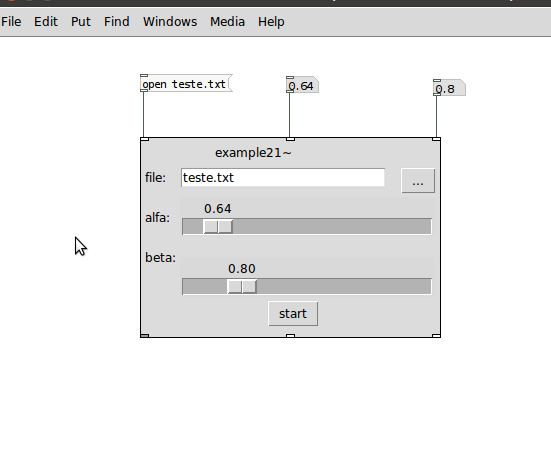
\includegraphics[width=0.7\textwidth]{example21}
	\caption{External com GUI e comandos}
\end{figure}



% ----------------------------------------------------------------------------
% ORIENTAÇÃO A OBJETOS
% ----------------------------------------------------------------------------

\chapter{Orientação a Objetos}

Parte do texto foi retirada de http://www.katjaas.nl/pitchshift/soundtouch~.html.

Este cara é um exemplo de external que utiliza uma biblioteca OO:
http://pure-data.svn.sourceforge.net/viewvc/pure-data/trunk/externals/fftw/fftw~.c?revision=6017&view=markup
No caso, a bibliteca utilizada é a FFTW3. Outro exemplo é o PDCUDA do Drebs!

Outro exemplo que utilizad OO em external é o pixopencv.

http://pure-data.svn.sourceforge.net/viewvc/pure-data/trunk/externals/pix_opencv/

É possível criar externals utilizando C++ e orientação a objetos. A parte crítica de tal implementação é garantir que o PD consiga enxergar as funções dentro do objeto compilado do C++. É necessário pensar nisto não apenas como uma alternativa para criar externals em C++ mas também para utilizar bibliotecas C++ para a criação de externals. Utilizar estas bibliotecas torna necessário que a mesma seja compilada na forma como símbolos em C. Para garantir isto é necessário utilizar a definição extern "C".

TERMINAR ESTE EXEMPLO. COMO FAZER PARA O MAKEFILE FUNCIONAR TAMBÉM PARA ARQUIVOS .H e .CPP?


\begin{lstlisting}
extern "C" void example18_setup(void) {
    example18_class = class_new(gensym("example18"),
            (t_newmethod) example18_new, // Constructor
            0,
            sizeof (t_example18),
	    CLASS_NOINLET,
            0);
};
\end{lstlisting}

Usando o setup "externalizado" o mesmo passa a ser exportado e compilado em um objeto com esta função "visível". Deve ser o suficiente para compilar o external com sua API utilizando C++. Para compilar, usados um compilador C++ como o g++ do Linux.

\begin{lstlisting}
LINUXCFLAGS = -msse -DPD -DUNIX -DICECAST -O3 -funroll-loops -fomit-frame-pointer -fcheck-new \
    -Wall -W -Wshadow \
    -Wno-unused -Wno-parentheses -Wno-switch -fvisibility=hidden

LINUXINCLUDE =  -I ./include

	g++ $(LINUXCFLAGS) $(LINUXINCLUDE) -c *.cpp 
	g++ --export-dynamic -shared -o $*.pd_linux *.o -lc -lm -lstdc++ 
	strip --strip-unneeded $(NAME).pd_linux
	rm -f *.o ../$(NAME).pd_linux
\end{lstlisting}



% ----------------------------------------------------------------------------
% MISCELÂNEAS
% ----------------------------------------------------------------------------

\chapter{Miscelâneas}
Como saber se um objeto existe?
pd\_findbyclass

Exemplo: http://pure-data.svn.sourceforge.net/viewvc/pure-data/trunk/pd/src/d\_array.c?revision=10432\&view=markup 

Linha 82


post

error

sys\_getblksize();

sys\_getsr()


\end{document}

